\documentclass{article}
\usepackage[utf8]{inputenc}
\usepackage[left = 2cm, right = 2cm, bottom = 2cm, top = 2cm]{geometry}
\usepackage{graphicx}
\usepackage{float}
\usepackage[spanish]{babel}
\spanishdecimal{.}
\usepackage{hyperref}
\usepackage{appendix}
\usepackage{longtable}

\title{Estudio de Regresión Lineal en los Resultados de los Aspirantes a Ingeniería Biomédica en la Universidad Autónoma de Chihuahua}
\author{Gerardo Pérez}
\date{Octubre 2020}

\begin{document}

\maketitle

\section{Introducción}

En el presente estudio se pretende obtener, de forma certera, cuáles apartados del examen de admisión y diagnóstico son más relevantes para determinar el puntaje global y con éste, a su vez, determinar si el aspirante a Ingeniería Biomédica (IB) será aceptado en la Universidad Autónoma de Chihuahua (UACh) o no.

Con los resultados obtenidos se pretende dar una retroalimentación a aquellos apirantes que quedaron fuera del proceso de selección, así como a aquellos estudiantes de nivel medio superior con pretenciones de ingresar a la carrera de IB.


\section{Planteamiento del Problema}

Para llevar a cabo este estudio, se tomaron en cuenta 9 de los 10 aspectos que se muestran en los resultados de admisión, ignorando el índice CENEVAL (ICNE) por la nula información que se obtendría tras las mediciones con este estandar.

Las variables tomadas en cuenta para el estudio se dividen en dos: aquellas que pertenecen al examen de admisión e impactan directamente al ICNE y a aquellas que pertenecen al examen de diagnóstico, quienes en suma con las variables del examen de admisión arrojan el puntaje global. Las variables pertenecientes al examen de admisión fueron los puntajes en el apartado de pensamiento matemático (PMA), pensamiento analítico (PAN), estructura de la lengua (ELE) y comprensión lectora (CLE); mientras que en el apartado del examen de diagnóstico se encuentra el puntaje en matemáticas (MAT), biología (BIO), lenguaje escrito (LES) e inglés (ING).

Para una mejor visualización de los resultados, a cada apartado del examen de admisión le fue asignada una variable, siendo PMA representado por $r$, PAN por $s$, ELE por $t$, CLE por $u$, MAT por $v$, BIO por $w$, LES por $x$ e ING por $z$.

Dado el tipo de examen presentado, en el que a mayor cantidad de reactivos acertados se obtendrá un mayor puntaje en el apartado y a su vez esto representa un mayor puntaje global, todas las ecuaciones presentadas tendrán la característica de ser directas y positivas, por lo cual esto será obviado en el análisis siguiente. Dicho análisis se realizó bajo un nivel de confianza del 95\%.


\section{Datos}

Los datos utilizados para realizar el presente estudio fueron obtenidos de uno de los apartados de la página oficial de la Universidad Autónoma de Chihuahua: \url{https://listas.uach.mx/}.

Por cuestión de espacio, sólo se mostrarán las primeras 15 tuplas en esta sección en el cuadro \ref{IB_PUESTOS}. Los datos completos utilizados para este estudio pueden encontrarse en el apartado de apéndices (ver apéndice A) o en la página citada previamente.

\begin{table}[H]
\centering
\begin{tabular}{c|c|c|c|c|c|c|c|c|c|}
\cline{2-10}
\multicolumn{1}{l|}{} & \textbf{PMA} & \textbf{PAN} & \textbf{ELE} & \textbf{CLE} & \textbf{MAT} & \textbf{BIO} & \textbf{LES} & \textbf{ING} & \textbf{GLOBAL} \\ \hline
\multicolumn{1}{|c|}{1}  & 1300 & 1276 & 1276 & 1204 & 1300 & 1210 & 1270 & 1300 & 1266 \\ \hline
\multicolumn{1}{|c|}{2}  & 1300 & 1204 & 1300 & 1204 & 1270 & 1270 & 1300 & 1270 & 1260 \\ \hline
\multicolumn{1}{|c|}{3}  & 1276 & 1252 & 1276 & 1204 & 1300 & 1240 & 1270 & 1270 & 1257 \\ \hline
\multicolumn{1}{|c|}{4}  & 1300 & 1252 & 1252 & 1276 & 1210 & 1240 & 1210 & 1210 & 1254 \\ \hline
\multicolumn{1}{|c|}{5}  & 1300 & 1204 & 1276 & 1252 & 1210 & 1210 & 1270 & 1270 & 1253 \\ \hline
\multicolumn{1}{|c|}{6}  & 1276 & 1276 & 1276 & 1204 & 1300 & 1210 & 1210 & 1240 & 1253 \\ \hline
\multicolumn{1}{|c|}{7}  & 1252 & 1276 & 1276 & 1252 & 1240 & 1210 & 1150 & 1210 & 1246 \\ \hline
\multicolumn{1}{|c|}{8}  & 1276 & 1252 & 1228 & 1276 & 1210 & 1210 & 1180 & 1240 & 1244 \\ \hline
\multicolumn{1}{|c|}{9}  & 1300 & 1252 & 1276 & 1228 & 1300 & 1300 & 1120 & 1060 & 1243 \\ \hline
\multicolumn{1}{|c|}{10} & 1276 & 1204 & 1252 & 1228 & 1210 & 1270 & 1210 & 1300 & 1242 \\ \hline
\multicolumn{1}{|c|}{11} & 1276 & 1252 & 1276 & 1084 & 1300 & 1270 & 1270 & 1300 & 1241 \\ \hline
\multicolumn{1}{|c|}{12} & 1276 & 1252 & 1252 & 1228 & 1210 & 1150 & 1180 & 1300 & 1239 \\ \hline
\multicolumn{1}{|c|}{13} & 1252 & 1252 & 1228 & 1132 & 1270 & 1300 & 1270 & 1300 & 1237 \\ \hline
\multicolumn{1}{|c|}{14} & 1276 & 1180 & 1252 & 1228 & 1210 & 1180 & 1240 & 1300 & 1234 \\ \hline
\multicolumn{1}{|c|}{15} & 1300 & 1228 & 1156 & 1228 & 1270 & 1180 & 1210 & 1300 & 1232 \\ \hline
\end{tabular}

\caption{Primeros 15 puestos del examen de admisión a Ingeniería Biomédica Agosto 2020.}
\label{IB_PUESTOS}
\end{table}

\section{Análisis de Resultados}

En esta sección se desglosará el análisis obtenido en cada una de las variables tomadas en cuenta para determinar el puntaje final o global que determina el ingreso o no de los aspirantes a la carrera de Ingeniería Biomédica ofrecida por la Universidad Autónoma de Chihuahua.

Esta sección estará dividida entonces en ocho subsecciones, éstas acorde a los aspectos evaluados, haciendo una comparativa individual con el puntaje global.

\subsection{GLOBAL-PMA}

El pensamiento matemático es el primer indicador que influye en el puntaje global del examen de admisión de la UACh. El comportamiento de la relación entre el puntaje global y el pensamiento matemático puede ser descrito mediante la ecuación \ref{PMA} que explica el comportamiento de estas dos variables en un $68.7\%$. Mientras que el índice de correlación se mantiene en $0.8288$, demostrando que la relación entre el pensamiento matemático y el puntaje global es muy fuerte.

\begin{equation}
    y = 317.9 + 0.6972r
    \label{PMA}
\end{equation}

Si se analiza el cuadro del análisis de varianza presente en la figura \ref{fig:AV_PMA} se podrá observar que la suma de cuadrados de los errores aporta más a la suma de cuadrados total que la suma de cuadrados de los errores, por lo que se encuentra dentro del intervalo de confianza propuesto.

\begin{figure}[H]
    \centering
    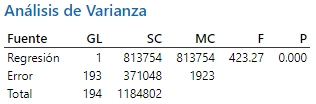
\includegraphics{PMA/AV_PMA.png}
    \caption{Análisis de varianza del puntaje global respecto al pensamiento matemático.}
    \label{fig:AV_PMA}
\end{figure}

Se puede apreciar en el diagrama de dispersión de la figura \ref{fig:G1_PMA} que la relación entre las variables es directa y positiva, lo que indicara que a medida que el valor del puntaje en PMA incrementa, también tiende a hacerlo el puntaje global.

\begin{figure}[H]
    \centering
    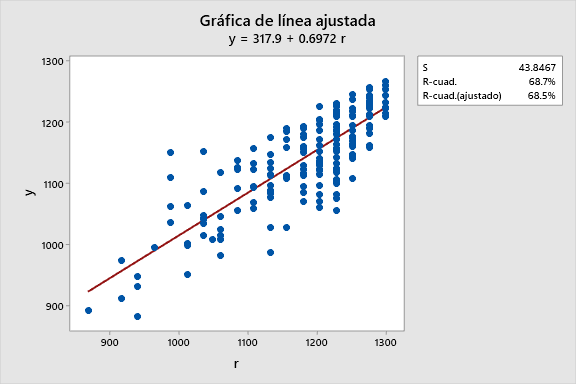
\includegraphics[scale = 0.66]{PMA/G1_PMA.png}
    \caption{Diagrama de dispersión puntaje global vs pensamiento matemático}
    \label{fig:G1_PMA}
\end{figure}

En la figura \ref{fig:G2_PMA} se puede observar cómo se distribuyen los residuos, donde podemos observar que se distribuyen de manera normal. Lo anterior indica que el supuesto de homocedasticidad se cumple y la ecuación de regresión lineal es válida para describir el comportamiento entre el puntaje del pensamiento matemático y el puntaje global.

\begin{figure}[H]
    \centering
    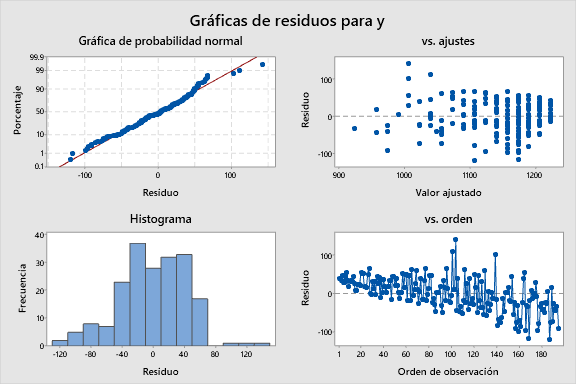
\includegraphics[scale = 0.66]{PMA/G2_PMA.png}
    \caption{Gráfica 4 en 1 de los residuos.}
    \label{fig:G2_PMA}
\end{figure}

\subsection{GLOBAL-PAN}

El pensamiento analítico es uno de los indicadores que influyen en el puntaje global del examen de admisión de la UACh. El comportamiento de la relación entre las variables puede ser descrito mediante la ecuación \ref{PAN} que explica el comportamiento de estas dos variables en un $68.2\%$. El índice de correlación entre estas dos variables es de $0.8258$ haciendo de la relación de las variables una muy fuerte.

\begin{equation}
    y = 317.9 + 0.6972r
    \label{PAN}
\end{equation}

Al observar la figura \ref{fig:AV_PAN} se puede notar inmediatamente que la suma de cuadrados de la regresión aporta más al total que la suma de cuadrados del error.

\begin{figure}[H]
    \centering
    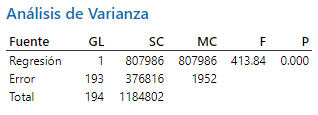
\includegraphics{PAN/AV_PAN.png}
    \caption{Análisis de varianza del puntaje global respecto al pensamiento analítico.}
    \label{fig:AV_PAN}
\end{figure}

Por otro lado, se puede apreciar en el diagrama de dispersión de la figura \ref{fig:G1_PAN} que la relación entre las variables es directa y positiva, lo que indicaría, como se indicó en la sección del planteamiento del problema, que a medida que el valor del puntaje en PAN incrementa, también tiende a hacerlo el puntaje global.

\begin{figure}[H]
    \centering
    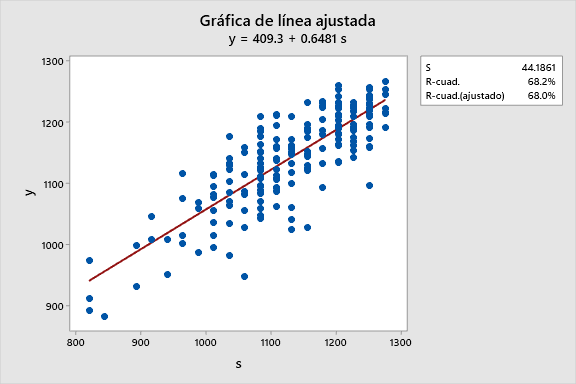
\includegraphics[scale = 0.66]{PAN/G1_PAN.png}
    \caption{Diagrama de dispersión puntaje global vs pensamiento analítico}
    \label{fig:G1_PAN}
\end{figure}

En la figura \ref{fig:G2_PAN} se puede observar cómo se distribuyen los residuos, donde podemos observar que se distribuyen de manera normal. Lo anterior indica que el supuesto de homocedasticidad se cumple y la ecuación de regresión lineal es válida para describir el comportamiento entre el puntaje del pensamiento analítico y el puntaje global.

\begin{figure}[H]
    \centering
    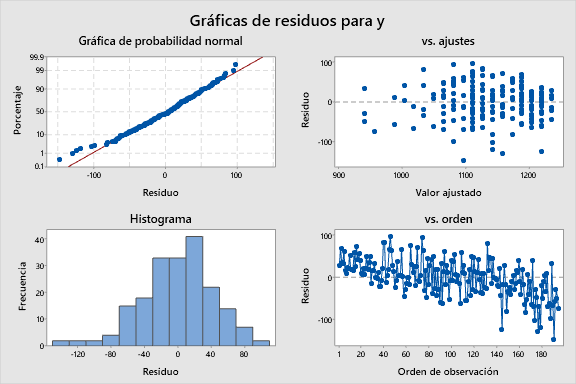
\includegraphics[scale = 0.66]{PAN/G2_PAN.png}
    \caption{Gráfica 4 en 1 de los residuos.}
    \label{fig:G2_PAN}
\end{figure}

\subsection{GLOBAL-ELE}

El puntaje en estructura del lenguaje es otro de los aspectos a analizar debido a su influencia en el puntaje global del examen de admisión de la UACh. El comportamiento de la relación entre el puntaje global y la estructura del lenguaje puede ser descrito mediante la ecuación \ref{ELE} que explica el comportamiento de estas dos variables en un $65.3\%$. Mientras que el índice de correlación se mantiene en $0.8080$, demostrando que la relación entre la estructura del lenguaje y el puntaje global es muy fuerte, aunque un tanto menor a el PMA y el PAN.

\begin{equation}
    y = 307.0 + 0.7234t
    \label{ELE}
\end{equation}

Al observar la figura \ref{fig:AV_ELE} se puede notar inmediatamente que la suma de cuadrados de la regresión aporta más al total que la suma de cuadrados del error.

\begin{figure}[H]
    \centering
    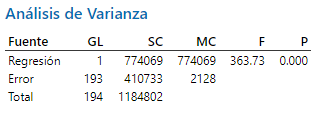
\includegraphics{ELE/AV_ELE.png}
    \caption{Análisis de varianza del puntaje global respecto la estructura de la lengua.}
    \label{fig:AV_ELE}
\end{figure}

Por otro lado, se puede apreciar en el diagrama de dispersión de la figura \ref{fig:G1_ELE} que la relación entre las variables es directa y positiva, lo que indica que a medida que el valor del puntaje en ELE incrementa, también tiende a hacerlo el puntaje global.

\begin{figure}[H]
    \centering
    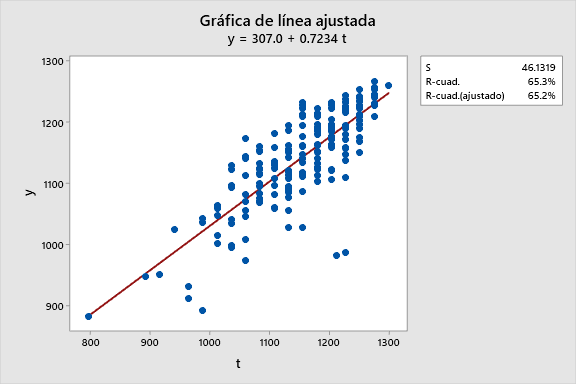
\includegraphics[scale = 0.66]{ELE/G1_ELE.png}
    \caption{Diagrama de dispersión puntaje global vs estructura de la lengua}
    \label{fig:G1_ELE}
\end{figure}

En la figura \ref{fig:G2_ELE} se puede observar cómo se distribuyen los residuos, donde podemos observar que se distribuyen de manera normal. Lo anterior indica que el supuesto de homocedasticidad se cumple y la ecuación de regresión lineal es válida para describir el comportamiento entre el puntaje del pensamiento analítico y el puntaje global.

\begin{figure}[H]
    \centering
    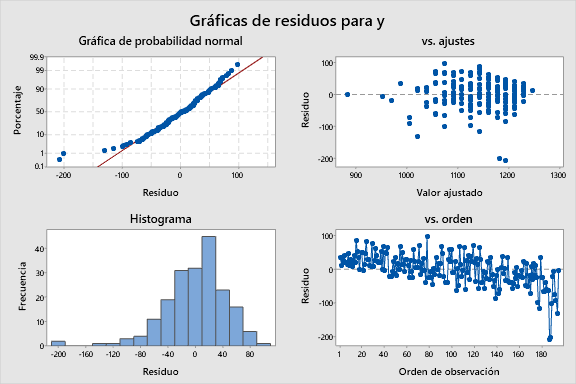
\includegraphics[scale = 0.66]{ELE/G2_ELE.png}
    \caption{Gráfica 4 en 1 de los residuos.}
    \label{fig:G2_ELE}
\end{figure}

\subsection{GLOBAL-CLE}

El puntaje en comprensión lectora es otro de los aspectos a analizar debido a su influencia en el puntaje global del examen de admisión de la UACh. Este es el último de los aspectos considerados directamente en el examen CENEVAL. El comportamiento de la relación entre el puntaje global y la estructura del lenguaje puede ser descrito mediante la ecuación \ref{CLE} que explica el comportamiento de estas dos variables en un $56.7\%$. Mientras que el índice de correlación se mantiene en $0.753$, demostrando que la relación entre la comprensión lectora y el puntaje global es fuerte. Para este punto, la relación con el puntaje global comienza a mermar.

\begin{equation}
    y = 439.8 + 0.6246u
    \label{CLE}
\end{equation}

Al observar la figura \ref{fig:AV_CLE} se puede notar inmediatamente que la suma de cuadrados de la regresión aporta más al total que la suma de cuadrados del error.

\begin{figure}[H]
    \centering
    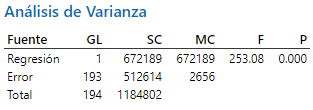
\includegraphics{CLE/AV_CLE.png}
    \caption{Análisis de varianza del puntaje global respecto a la comprensión lectora.}
    \label{fig:AV_CLE}
\end{figure}

El diagrama de dispersión de la figura \ref{fig:G1_CLE} muestra que la relación entre las variables es directa y positiva, aunque el comportamiento de los valores es bastante más complicado que los diagramas de dispersión que hacían uso del PMA, PAN y ELE.

\begin{figure}[H]
    \centering
    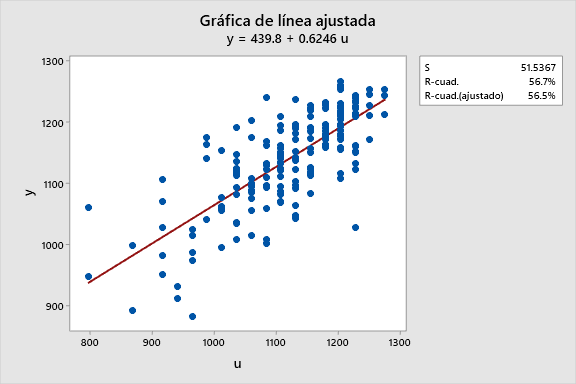
\includegraphics[scale = 0.66]{CLE/G1_CLE.png}
    \caption{Diagrama de dispersión puntaje global vs comprensión lectora.}
    \label{fig:G1_CLE}
\end{figure}

En la figura \ref{fig:G2_CLE} se puede observar cómo se distribuyen los residuos, donde podemos observar que se distribuyen de manera normal. Lo anterior indica que el supuesto de homocedasticidad se cumple y la ecuación de regresión lineal es válida para describir el comportamiento entre el puntaje del pensamiento analítico y el puntaje global.

\begin{figure}[H]
    \centering
    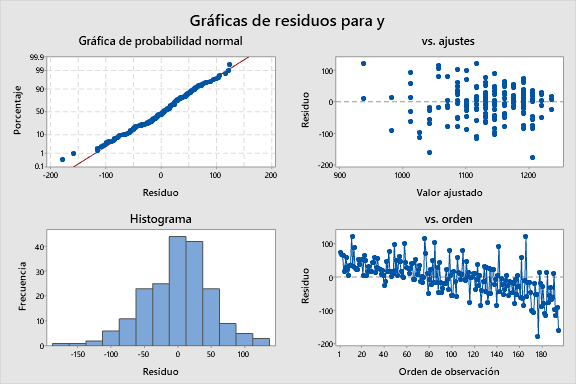
\includegraphics[scale = 0.66]{CLE/G2_CLE.png}
    \caption{Gráfica 4 en 1 de los residuos.}
    \label{fig:G2_CLE}
\end{figure}

\subsection{GLOBAL-MAT}

En este punto se comienzan a analizar la relación entre los puntajes del examen de diagnóstico en sus diferentes etapas, en este caso matemáticas, para determinar la influencia en el puntaje global.

La relación entre estas dos variables puede representarse mediante la ecuación \ref{MAT} que explica en un $51.7\%$ la relación entre el puntaje global y el puntaje en matemáticas. La correlación existente entre estas dos variables es de $0.72$, lo que indica una correlación fuerte.

\begin{equation}
    y = 512.2 + 0.5506v
    \label{MAT}
\end{equation}

El análisis de varianza de la figura \ref{fig:AV_MAT} muestra una predominancia en la suma de cuadrados de la regresión respecto a la suma de cuadrados del error, aunque es menos clara que en aquellas instancias pertenecientes al examen CENEVAL.

\begin{figure}[H]
    \centering
    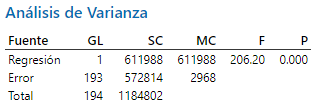
\includegraphics{MAT/AV_MAT.png}
    \caption{Análisis de varianza del puntaje global respecto a matemáticas.}
    \label{fig:AV_MAT}
\end{figure}

Tal y como se expresa gracias al análisis de varianza, la distribución de los puntajes a lo largo de la gráfica mostrada en la figura \ref{fig:G1_MAT} no concuerdan de una manera muy acertada con la recta de la regresión lineal.

\begin{figure}[H]
    \centering
    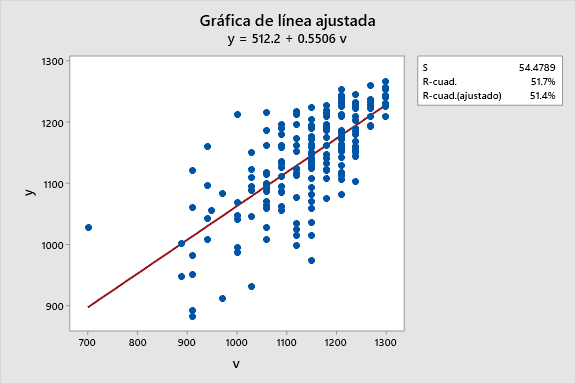
\includegraphics[scale = 0.66]{MAT/G1_MAT.png}
    \caption{Diagrama de dispersión puntaje global vs matemáticas.}
    \label{fig:G1_MAT}
\end{figure}

En la figura \ref{fig:G2_MAT} se puede observar cómo se distribuyen los residuos, donde podemos observar que se distribuyen de manera normal. Lo anterior indica que el supuesto de homocedasticidad se cumple y la ecuación de regresión lineal es válida para describir el comportamiento entre el puntaje del pensamiento analítico y el puntaje global.

\begin{figure}[H]
    \centering
    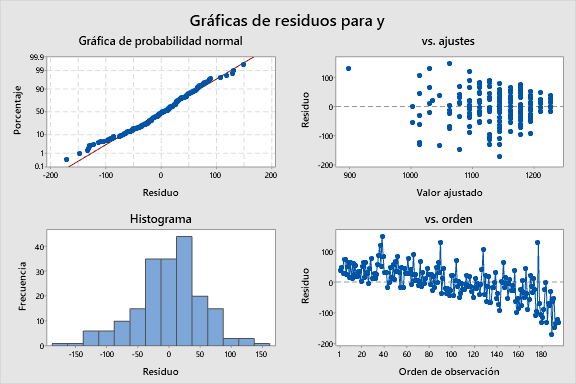
\includegraphics[scale = 0.66]{MAT/G2_MAT.png}
    \caption{Gráfica 4 en 1 de los residuos.}
    \label{fig:G2_MAT}
\end{figure}

\subsection{GLOBAL-BIO}

Biología es uno de los apartados considerados recientemente para la determinación en el ingreso o no de los aspirantes. La ecuación \ref{BIO} explica en un $54.1\%$ la relación entre el puntaje en biología y el puntaje global, mientras que un índice de correlación de $0.735$ indica que tiene una mayor relación con el puntaje global que el puntaje en matemáticas.

\begin{equation}
    y = 566.6 + 0.5176w
    \label{BIO}
\end{equation}

El análisis de varianza de la figura \ref{fig:AV_BIO} muestra un mayor aporte de la suma de cuadrados de la regresión que de los residuos, lo que indica que se mantiene dentro del intervalo de confianza.

\begin{figure}[H]
    \centering
    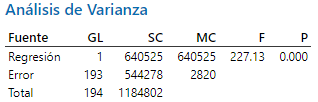
\includegraphics{BIO/AV_BIO.png}
    \caption{Análisis de varianza del puntaje global respecto a biología.}
    \label{fig:AV_BIO}
\end{figure}

El diagrama de dispersión presentado en la figura \ref{fig:G1_BIO} muestra el comportamiento positivo y directo entre ambas variables.

\begin{figure}[H]
    \centering
    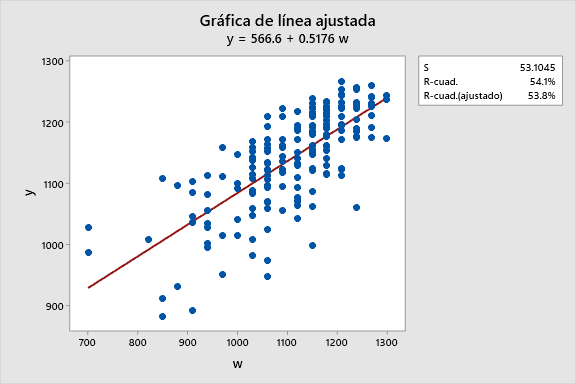
\includegraphics[scale = 0.66]{BIO/G1_BIO.png}
    \caption{Diagrama de dispersión puntaje global vs biología.}
    \label{fig:G1_BIO}
\end{figure}

En la figura \ref{fig:G2_BIO} se puede observar cómo se distribuyen los residuos, donde podemos observar que se distribuyen de manera normal. Lo anterior indica que el supuesto de homocedasticidad se cumple y la ecuación de regresión lineal es válida para describir el comportamiento entre el puntaje del pensamiento analítico y el puntaje global.

\begin{figure}[H]
    \centering
    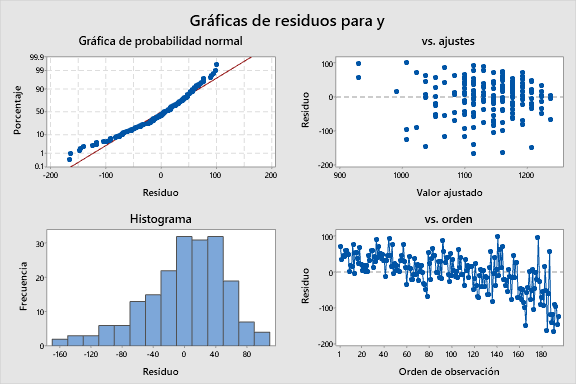
\includegraphics[scale = 0.66]{BIO/G2_BIO.png}
    \caption{Gráfica 4 en 1 de los residuos.}
    \label{fig:G2_BIO}
\end{figure}

\subsection{GLOBAL-LES}

El lenguaje escrito es la penúltima variable considerada en este estudio como referencia para el puntaje global. En este caso, la ecuación \ref{LES} explica el comportamiento de los resultados en un $51.8\%$, además de una correlación de $0.7197$ que lo deja como una relación fuerte entre las variables. 

\begin{equation}
    y = 635.3 + 0.4562x
    \label{LES}
\end{equation}

La figura \ref{fig:AV_LES} muestra el análisis de varianza del puntaje global y el puntaje LES, donde predomina por poco el aporte de la suma de cuadrados de la regresión al total en comparación a la suma de cuadrados del error.

\begin{figure}[H]
    \centering
    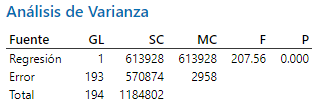
\includegraphics{LES/AV_LES.png}
    \caption{Análisis de varianza del puntaje global respecto al lenguaje escrito.}
    \label{fig:AV_LES}
\end{figure}

La gráfica de dispersión de la figura \ref{fig:G1_LES} hace notar la relación un tanto pobre entre las variables, ya que a pesar de tener una tendencia a incrementar el puntaje global cuando incrementa el puntaje LES, existe una mayor presencia de anomalías.

\begin{figure}[H]
    \centering
    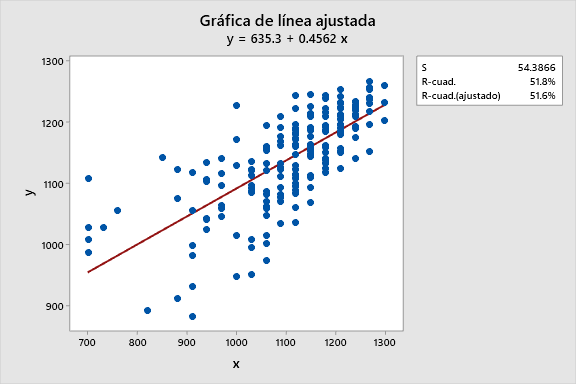
\includegraphics[scale = 0.66]{LES/G1_LES.png}
    \caption{Diagrama de dispersión puntaje global vs lenguaje escrito.}
    \label{fig:G1_LES}
\end{figure}

En la figura \ref{fig:G2_LES} se puede observar cómo se distribuyen los residuos, donde podemos observar que se distribuyen de manera normal. Lo anterior indica que el supuesto de homocedasticidad se cumple y la ecuación de regresión lineal es válida para describir el comportamiento entre el puntaje del pensamiento analítico y el puntaje global.

\begin{figure}[H]
    \centering
    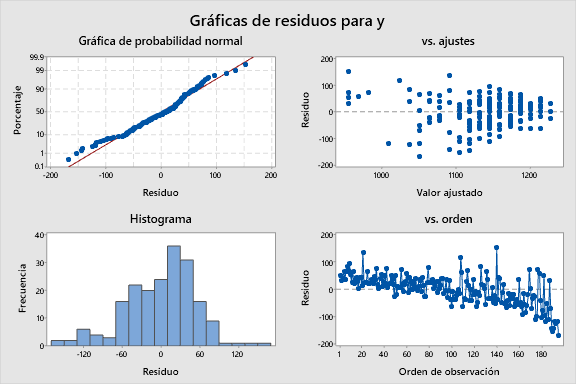
\includegraphics[scale = 0.66]{LES/G2_LES.png}
    \caption{Gráfica 4 en 1 de los residuos.}
    \label{fig:G2_LES}
\end{figure}

\subsection{GLOBAL-ING}

El apartado de inglés tiene un comportamiento descrito por la ecuación \ref{ING}, que explica en un $43.6\%$ el comportamiento del puntaje de inglés con el del puntaje global. La correlación entre las variables en este apartado es bastante pobre en comparación a los anteriores, ya que la gran mayoría presenta puntajes altos en esta categoría que no hacen justicia al puntaje global, esta correlación es de $0.6603$ lo que la sitúa en una correlación moderada.

\begin{equation}
    y = 721.7 + 0.3643
    \label{ING}
\end{equation}

El análisis de varianza presente en la figura \ref{fig:AV_ING} muestra un aporte mayor de la suma de cuadrados del error respecto a la suma de cuadrados de la regresión al total. No obstante, aún así se mantiene entre el intervalo de confianza propuesto.

\begin{figure}[H]
    \centering
    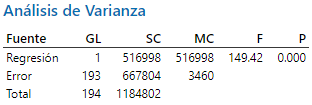
\includegraphics{ING/AV_ING.png}
    \caption{Análisis de varianza del puntaje global respecto a inglés.}
    \label{fig:AV_ING}
\end{figure}

Como se mencionó previamente y se puede observar en el diagrama de dispersión de la figura \ref{fig:G1_ING}, los puntajes altos en inglés no representan, necesariamente, un buen puntaje global.

\begin{figure}[H]
    \centering
    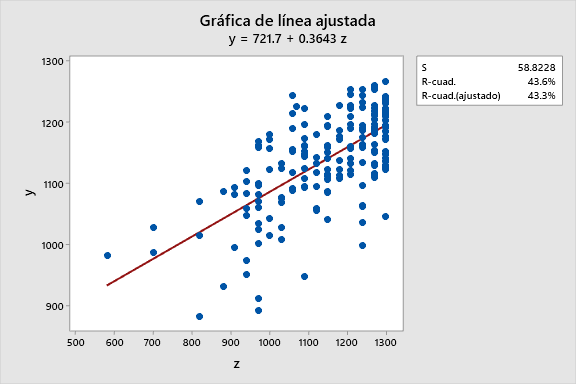
\includegraphics[scale = 0.66]{ING/G1_ING.png}
    \caption{Diagrama de dispersión puntaje global vs inglés}
    \label{fig:G1_ING}
\end{figure}

En la figura \ref{fig:G2_ING} se puede observar cómo se distribuyen los residuos, donde podemos observar que se distribuyen de manera normal. Lo anterior indica que el supuesto de homocedasticidad se cumple y la ecuación de regresión lineal es válida para describir el comportamiento entre el puntaje del pensamiento analítico y el puntaje global.

\begin{figure}[H]
    \centering
    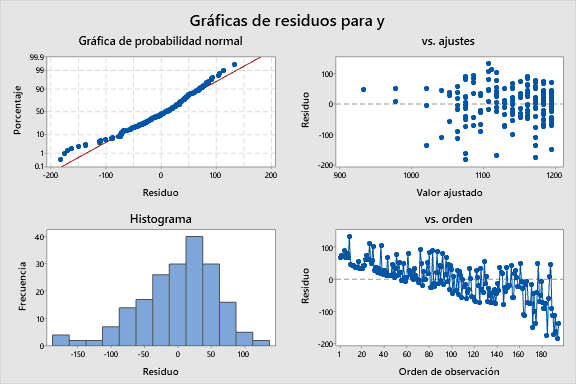
\includegraphics[scale = 0.66]{ING/G2_ING.png}
    \caption{Gráfica 4 en 1 de los residuos.}
    \label{fig:G2_ING}
\end{figure}

\section{Análisis Global}

Tras un proceso de análisis individual en cada uno de los parámetros relacionados con el puntaje global se puede observar, como se previno en el planteamiento del problema, que cada uno de estos puntajes se relacionan de manera directa y positiva con el puntaje global, por lo que en criterios amplios un buen puntaje individual implica un buen puntaje global.

Por otro lado, se puede resumir de cada uno de los gráficos de los residuos presentados a lo largo del estudio que estos no presentan patrón alguno que impida realizar el análisis al infringir uno de los supuestos del modelo. En otras palabras, se distribuyen de manera normal.

Es de recalcar que tras observar el nivel de correlación presentado en cada uno de los parámetros, se puede determinar que a pesar del pensamiento intuitivo de centrarse en el estudio de biología para incrementar el puntaje, este parámetro y todos los pertenecientes al apartado del examen de diagnóstico influyen más bien poco en comparación con los puntajes obtenidos en el apartado del examen de admisión.

Se puede observar que los dos puntajes individuales que influyeron en mayor medida en los puntajes globales son el puntaje en el apartado de pensamiento matemático, con una correlación de $0.8288$ con el puntaje global y el apartado del pensamiento analítico, con una correlación de $0.8258$ respecto al puntaje global, siendo el menos influyente el puntaje obtenido en inglés con una correlación mínima de $0.6603$ respecto al puntaje global.

A pesar de tener una correlación menor a los puntajes obtenidos del examen de admisión, se puede observar que el puntaje en biología es el de mayor correlación con el puntaje global del apartado de diagnóstico, lo que indica que aquellos aspirantes seleccionados se centraron en el estudio de biología, aunque esto no mejoraba tanto sus posibilidades de ser seleccionados.

En conclusión se puede decir que los dos aspectos que más influyen en la selección o no, es decir, los aspectos que diferencían a aquellos que fueron seleccionados de los que no se centran en el pensamiento matemático y el pensamiento lógico. La recomendación para los futuros aspirantes es centrar su estudio en los parámetros propiamente pertenecientes al ICNE, haciéndo énfasis en estos últimos dos aspectos y en menor medida a aquellos parámetros que afectan directamente al examen de diagnóstico.

\newpage

\appendix

\section{Lista de resultados Ingeniero Biomédico Agosto 2020}

\begin{table}[H]
\centering
\begin{tabular}{c|c|c|c|c|c|c|c|c|c|}
\cline{2-10}
 & \textbf{PMA} & \textbf{PAN} & \textbf{ELE} & \textbf{CLE} & \textbf{MAT} & \textbf{BIO} & \textbf{LES} & \textbf{ING} & \textbf{GLOBAL} \\ \hline
\multicolumn{1}{|c|}{1}   & 1300 & 1276 & 1276 & 1204 & 1300 & 1210 & 1270 & 1300 & 1266 \\ \hline
\multicolumn{1}{|c|}{2}   & 1300 & 1204 & 1300 & 1204 & 1270 & 1270 & 1300 & 1270 & 1260 \\ \hline
\multicolumn{1}{|c|}{3}   & 1276 & 1252 & 1276 & 1204 & 1300 & 1240 & 1270 & 1270 & 1257 \\ \hline
\multicolumn{1}{|c|}{4}   & 1300 & 1252 & 1252 & 1276 & 1210 & 1240 & 1210 & 1210 & 1254 \\ \hline
\multicolumn{1}{|c|}{5}   & 1300 & 1204 & 1276 & 1252 & 1210 & 1210 & 1270 & 1270 & 1253 \\ \hline
\multicolumn{1}{|c|}{6}   & 1276 & 1276 & 1276 & 1204 & 1300 & 1210 & 1210 & 1240 & 1253 \\ \hline
\multicolumn{1}{|c|}{7}   & 1252 & 1276 & 1276 & 1252 & 1240 & 1210 & 1150 & 1210 & 1246 \\ \hline
\multicolumn{1}{|c|}{8}   & 1276 & 1252 & 1228 & 1276 & 1210 & 1210 & 1180 & 1240 & 1244 \\ \hline
\multicolumn{1}{|c|}{9}   & 1300 & 1252 & 1276 & 1228 & 1300 & 1300 & 1120 & 1060 & 1243 \\ \hline
\multicolumn{1}{|c|}{10}  & 1276 & 1204 & 1252 & 1228 & 1210 & 1270 & 1210 & 1300 & 1242 \\ \hline
\multicolumn{1}{|c|}{11}  & 1276 & 1252 & 1276 & 1084 & 1300 & 1270 & 1270 & 1300 & 1241 \\ \hline
\multicolumn{1}{|c|}{12}  & 1276 & 1252 & 1252 & 1228 & 1210 & 1150 & 1180 & 1300 & 1239 \\ \hline
\multicolumn{1}{|c|}{13}  & 1252 & 1252 & 1228 & 1132 & 1270 & 1300 & 1270 & 1300 & 1237 \\ \hline
\multicolumn{1}{|c|}{14}  & 1276 & 1180 & 1252 & 1228 & 1210 & 1180 & 1240 & 1300 & 1234 \\ \hline
\multicolumn{1}{|c|}{15}  & 1300 & 1228 & 1156 & 1228 & 1270 & 1180 & 1210 & 1300 & 1232 \\ \hline
\multicolumn{1}{|c|}{16}  & 1300 & 1156 & 1204 & 1228 & 1270 & 1210 & 1240 & 1300 & 1232 \\ \hline
\multicolumn{1}{|c|}{17}  & 1276 & 1204 & 1228 & 1180 & 1240 & 1240 & 1300 & 1240 & 1232 \\ \hline
\multicolumn{1}{|c|}{18}  & 1276 & 1180 & 1276 & 1204 & 1240 & 1150 & 1210 & 1300 & 1231 \\ \hline
\multicolumn{1}{|c|}{19}  & 1276 & 1204 & 1204 & 1180 & 1300 & 1240 & 1210 & 1300 & 1230 \\ \hline
\multicolumn{1}{|c|}{20}  & 1228 & 1252 & 1204 & 1180 & 1210 & 1270 & 1270 & 1300 & 1230 \\ \hline
\multicolumn{1}{|c|}{21}  & 1228 & 1252 & 1276 & 1252 & 1180 & 1240 & 1000 & 1270 & 1228 \\ \hline
\multicolumn{1}{|c|}{22}  & 1228 & 1228 & 1252 & 1156 & 1270 & 1240 & 1240 & 1270 & 1228 \\ \hline
\multicolumn{1}{|c|}{23}  & 1276 & 1252 & 1204 & 1180 & 1180 & 1270 & 1240 & 1210 & 1227 \\ \hline
\multicolumn{1}{|c|}{24}  & 1276 & 1228 & 1156 & 1252 & 1240 & 1240 & 1240 & 1180 & 1227 \\ \hline
\multicolumn{1}{|c|}{25}  & 1276 & 1180 & 1228 & 1228 & 1240 & 1270 & 1150 & 1210 & 1225 \\ \hline
\multicolumn{1}{|c|}{26}  & 1228 & 1228 & 1228 & 1204 & 1300 & 1180 & 1240 & 1210 & 1225 \\ \hline
\multicolumn{1}{|c|}{27}  & 1204 & 1204 & 1252 & 1228 & 1210 & 1210 & 1240 & 1070 & 1225 \\ \hline
\multicolumn{1}{|c|}{28}  & 1300 & 1180 & 1252 & 1228 & 1150 & 1150 & 1210 & 1240 & 1224 \\ \hline
\multicolumn{1}{|c|}{29}  & 1300 & 1276 & 1156 & 1180 & 1270 & 1150 & 1210 & 1210 & 1223 \\ \hline
\multicolumn{1}{|c|}{30}  & 1252 & 1228 & 1252 & 1180 & 1270 & 1240 & 1240 & 1090 & 1223 \\ \hline
\multicolumn{1}{|c|}{31}  & 1276 & 1228 & 1228 & 1156 & 1240 & 1180 & 1180 & 1300 & 1223 \\ \hline
\multicolumn{1}{|c|}{32}  & 1252 & 1204 & 1180 & 1228 & 1270 & 1210 & 1210 & 1270 & 1223 \\ \hline
\multicolumn{1}{|c|}{33}  & 1300 & 1252 & 1204 & 1204 & 1240 & 1090 & 1120 & 1270 & 1222 \\ \hline
\multicolumn{1}{|c|}{34}  & 1228 & 1252 & 1228 & 1156 & 1180 & 1180 & 1240 & 1300 & 1219 \\ \hline
\multicolumn{1}{|c|}{35}  & 1252 & 1228 & 1228 & 1204 & 1120 & 1120 & 1270 & 1270 & 1218 \\ \hline
\multicolumn{1}{|c|}{36}  & 1228 & 1276 & 1228 & 1204 & 1060 & 1150 & 1180 & 1300 & 1216 \\ \hline
\multicolumn{1}{|c|}{37}  & 1300 & 1276 & 1180 & 1228 & 1180 & 1180 & 1150 & 1060 & 1215 \\ \hline

\end{tabular}
\end{table}

\begin{table}
\centering
\begin{tabular}{c|c|c|c|c|c|c|c|c|c|}
\cline{2-10}
& \textbf{PMA} & \textbf{PAN} & \textbf{ELE} & \textbf{CLE} & \textbf{MAT} & \textbf{BIO} & \textbf{LES} & \textbf{ING} & \textbf{GLOBAL} \\ \hline
\multicolumn{1}{|c|}{38}  & 1228 & 1252 & 1252 & 1204 & 1000 & 1150 & 1240 & 1270 & 1213 \\ \hline
\multicolumn{1}{|c|}{39}  & 1276 & 1204 & 1156 & 1228 & 1120 & 1180 & 1210 & 1300 & 1212 \\ \hline
\multicolumn{1}{|c|}{40}  & 1228 & 1108 & 1252 & 1276 & 1210 & 1180 & 1150 & 1270 & 1212 \\ \hline
\multicolumn{1}{|c|}{41}  & 1252 & 1108 & 1180 & 1252 & 1210 & 1270 & 1210 & 1270 & 1211 \\ \hline
\multicolumn{1}{|c|}{42}  & 1276 & 1252 & 1180 & 1156 & 1210 & 1180 & 1090 & 1300 & 1210 \\ \hline
\multicolumn{1}{|c|}{43}  & 1252 & 1228 & 1156 & 1204 & 1300 & 1150 & 1240 & 1150 & 1210 \\ \hline
\multicolumn{1}{|c|}{44}  & 1252 & 1204 & 1276 & 1108 & 1270 & 1060 & 1210 & 1300 & 1210 \\ \hline
\multicolumn{1}{|c|}{45}  & 1228 & 1132 & 1276 & 1204 & 1180 & 1150 & 1210 & 1300 & 1210 \\ \hline
\multicolumn{1}{|c|}{46}  & 1228 & 1084 & 1276 & 1228 & 1240 & 1210 & 1150 & 1300 & 1210 \\ \hline
\multicolumn{1}{|c|}{47}  & 1300 & 1132 & 1252 & 1204 & 1240 & 1090 & 1180 & 1210 & 1209 \\ \hline
\multicolumn{1}{|c|}{48}  & 1204 & 1180 & 1204 & 1204 & 1150 & 1240 & 1210 & 1270 & 1204 \\ \hline
\multicolumn{1}{|c|}{49}  & 1204 & 1204 & 1252 & 1060 & 1240 & 1180 & 1300 & 1300 & 1203 \\ \hline
\multicolumn{1}{|c|}{50}  & 1228 & 1252 & 1180 & 1180 & 1120 & 1210 & 1120 & 1210 & 1197 \\ \hline
\multicolumn{1}{|c|}{51}  & 1204 & 1228 & 1252 & 1132 & 1180 & 1180 & 1270 & 1090 & 1197 \\ \hline
\multicolumn{1}{|c|}{52}  & 1228 & 1156 & 1204 & 1204 & 1090 & 1210 & 1210 & 1270 & 1197 \\ \hline
\multicolumn{1}{|c|}{53}  & 1252 & 1204 & 1228 & 1108 & 1180 & 1210 & 1210 & 1150 & 1195 \\ \hline
\multicolumn{1}{|c|}{54}  & 1276 & 1204 & 1132 & 1132 & 1270 & 1150 & 1210 & 1240 & 1195 \\ \hline
\multicolumn{1}{|c|}{55}  & 1252 & 1204 & 1204 & 1180 & 1150 & 1120 & 1060 & 1300 & 1194 \\ \hline
\multicolumn{1}{|c|}{56}  & 1252 & 1108 & 1156 & 1204 & 1270 & 1150 & 1180 & 1300 & 1194 \\ \hline
\multicolumn{1}{|c|}{57}  & 1180 & 1204 & 1204 & 1204 & 1270 & 1060 & 1240 & 1150 & 1193 \\ \hline
\multicolumn{1}{|c|}{58}  & 1228 & 1276 & 1228 & 1036 & 1150 & 1150 & 1180 & 1270 & 1191 \\ \hline
\multicolumn{1}{|c|}{59}  & 1180 & 1252 & 1180 & 1132 & 1180 & 1180 & 1150 & 1300 & 1191 \\ \hline
\multicolumn{1}{|c|}{60}  & 1180 & 1228 & 1180 & 1156 & 1180 & 1270 & 1090 & 1270 & 1191 \\ \hline
\multicolumn{1}{|c|}{61}  & 1276 & 1204 & 1204 & 1156 & 1090 & 1180 & 1240 & 1060 & 1190 \\ \hline
\multicolumn{1}{|c|}{62}  & 1180 & 1204 & 1252 & 1180 & 1180 & 1120 & 1120 & 1210 & 1190 \\ \hline
\multicolumn{1}{|c|}{63}  & 1180 & 1228 & 1180 & 1156 & 1150 & 1180 & 1210 & 1240 & 1189 \\ \hline
\multicolumn{1}{|c|}{64}  & 1276 & 1084 & 1228 & 1132 & 1240 & 1240 & 1150 & 1210 & 1189 \\ \hline
\multicolumn{1}{|c|}{65}  & 1156 & 1156 & 1252 & 1132 & 1180 & 1240 & 1210 & 1270 & 1189 \\ \hline
\multicolumn{1}{|c|}{66}  & 1252 & 1180 & 1132 & 1204 & 1060 & 1210 & 1150 & 1270 & 1186 \\ \hline
\multicolumn{1}{|c|}{67}  & 1228 & 1156 & 1180 & 1204 & 1210 & 1120 & 1180 & 1180 & 1186 \\ \hline
\multicolumn{1}{|c|}{68}  & 1204 & 1228 & 1204 & 1108 & 1180 & 1210 & 1120 & 1240 & 1186 \\ \hline
\multicolumn{1}{|c|}{69}  & 1156 & 1156 & 1204 & 1180 & 1210 & 1150 & 1210 & 1270 & 1185 \\ \hline
\multicolumn{1}{|c|}{70}  & 1228 & 1084 & 1180 & 1156 & 1240 & 1240 & 1180 & 1300 & 1185 \\ \hline
\multicolumn{1}{|c|}{71}  & 1276 & 1204 & 1108 & 1132 & 1210 & 1150 & 1120 & 1270 & 1182 \\ \hline
\multicolumn{1}{|c|}{72}  & 1228 & 1204 & 1228 & 1204 & 1090 & 1180 & 1120 & 1000 & 1180 \\ \hline
\multicolumn{1}{|c|}{73}  & 1180 & 1180 & 1180 & 1180 & 1240 & 1150 & 1210 & 1120 & 1180 \\ \hline
\multicolumn{1}{|c|}{74}  & 1252 & 1036 & 1204 & 1204 & 1150 & 1180 & 1090 & 1300 & 1176 \\ \hline
\multicolumn{1}{|c|}{75}  & 1252 & 1084 & 1156 & 1180 & 1210 & 1240 & 1150 & 1180 & 1176 \\ \hline
\multicolumn{1}{|c|}{76}  & 1180 & 1228 & 1204 & 988  & 1210 & 1240 & 1240 & 1240 & 1175 \\ \hline
\multicolumn{1}{|c|}{77}  & 1132 & 1156 & 1252 & 1060 & 1180 & 1270 & 1240 & 1240 & 1175 \\ \hline
\multicolumn{1}{|c|}{78}  & 1252 & 1252 & 1060 & 1156 & 1120 & 1300 & 1120 & 1090 & 1173 \\ \hline
\multicolumn{1}{|c|}{79}  & 1228 & 1108 & 1228 & 1252 & 1150 & 1060 & 1000 & 1180 & 1172 \\ \hline
\multicolumn{1}{|c|}{80}  & 1204 & 1204 & 1228 & 1180 & 1150 & 1120 & 1120 & 1000 & 1172 \\ \hline
\multicolumn{1}{|c|}{81}  & 1156 & 1132 & 1204 & 1132 & 1210 & 1210 & 1120 & 1300 & 1172 \\ \hline
\multicolumn{1}{|c|}{82}  & 1156 & 1108 & 1228 & 1204 & 1150 & 1090 & 1120 & 1300 & 1171 \\ \hline
\multicolumn{1}{|c|}{83}  & 1252 & 1228 & 1252 & 1084 & 1240 & 1030 & 1090 & 970  & 1168 \\ \hline
\multicolumn{1}{|c|}{84}  & 1228 & 1084 & 1180 & 1180 & 1150 & 1060 & 1150 & 1240 & 1163 \\ \hline
\multicolumn{1}{|c|}{85}  & 1252 & 1204 & 1204 & 988  & 1210 & 1060 & 1120 & 1270 & 1163 \\ \hline
\multicolumn{1}{|c|}{86}  & 1276 & 1132 & 1132 & 1180 & 1090 & 1150 & 1090 & 1150 & 1162 \\ \hline
\multicolumn{1}{|c|}{87}  & 1204 & 1228 & 1180 & 1108 & 1180 & 1150 & 1180 & 970  & 1162 \\ \hline
\multicolumn{1}{|c|}{88}  & 1204 & 1132 & 1156 & 1228 & 1060 & 1090 & 1090 & 1240 & 1162 \\ \hline
\multicolumn{1}{|c|}{89}  & 1204 & 1204 & 1204 & 1084 & 1120 & 1180 & 1150 & 1090 & 1162 \\ \hline
\multicolumn{1}{|c|}{90}  & 1180 & 1252 & 1156 & 1180 & 940  & 1090 & 1120 & 1210 & 1161 \\ \hline
\end{tabular}
\end{table}

\begin{table}
\centering
\begin{tabular}{c|c|c|c|c|c|c|c|c|c|}
\cline{2-10}
& \textbf{PMA} & \textbf{PAN} & \textbf{ELE} & \textbf{CLE} & \textbf{MAT} & \textbf{BIO} & \textbf{LES} & \textbf{ING} & \textbf{GLOBAL} \\ \hline
\multicolumn{1}{|c|}{91}  & 1252 & 1108 & 1084 & 1228 & 1240 & 1180 & 1060 & 1090 & 1160 \\ \hline
\multicolumn{1}{|c|}{92}  & 1276 & 1252 & 1108 & 1204 & 1150 & 970  & 1060 & 970  & 1158 \\ \hline
\multicolumn{1}{|c|}{93}  & 1156 & 1132 & 1204 & 1180 & 1090 & 1030 & 1180 & 1240 & 1158 \\ \hline
\multicolumn{1}{|c|}{94}  & 1180 & 1060 & 1228 & 1180 & 1210 & 1090 & 1150 & 1150 & 1158 \\ \hline
\multicolumn{1}{|c|}{95}  & 1228 & 1180 & 1228 & 1108 & 1240 & 1060 & 1060 & 1000 & 1157 \\ \hline
\multicolumn{1}{|c|}{96}  & 1108 & 1108 & 1228 & 1156 & 1210 & 1060 & 1210 & 1210 & 1157 \\ \hline
\multicolumn{1}{|c|}{97}  & 1180 & 1132 & 1132 & 1204 & 1210 & 1150 & 1150 & 1060 & 1156 \\ \hline
\multicolumn{1}{|c|}{98}  & 1228 & 1228 & 1084 & 1012 & 1240 & 1180 & 1060 & 1270 & 1153 \\ \hline
\multicolumn{1}{|c|}{99}  & 1228 & 1156 & 1132 & 1132 & 1210 & 1030 & 1210 & 1060 & 1152 \\ \hline
\multicolumn{1}{|c|}{100} & 1204 & 1084 & 1084 & 1228 & 1120 & 1150 & 1270 & 1090 & 1152 \\ \hline
\multicolumn{1}{|c|}{101} & 1036 & 1156 & 1180 & 1228 & 1120 & 1060 & 1150 & 1300 & 1152 \\ \hline
\multicolumn{1}{|c|}{102} & 1180 & 1084 & 1180 & 1108 & 1240 & 1120 & 1210 & 1150 & 1151 \\ \hline
\multicolumn{1}{|c|}{103} & 1180 & 1060 & 1132 & 1156 & 1150 & 1150 & 1210 & 1270 & 1151 \\ \hline
\multicolumn{1}{|c|}{104} & 988  & 1132 & 1252 & 1228 & 1030 & 1120 & 1180 & 1270 & 1150 \\ \hline
\multicolumn{1}{|c|}{105} & 1252 & 1156 & 1156 & 1036 & 1180 & 1150 & 1150 & 1090 & 1148 \\ \hline
\multicolumn{1}{|c|}{106} & 1132 & 1132 & 1228 & 1108 & 1150 & 1000 & 1120 & 1300 & 1148 \\ \hline
\multicolumn{1}{|c|}{107} & 1252 & 1156 & 1060 & 1108 & 1240 & 1090 & 1150 & 1090 & 1144 \\ \hline
\multicolumn{1}{|c|}{108} & 1228 & 1228 & 1132 & 1132 & 1210 & 1030 & 850  & 1120 & 1142 \\ \hline
\multicolumn{1}{|c|}{109} & 1252 & 1036 & 1180 & 1108 & 1150 & 1120 & 970  & 1300 & 1141 \\ \hline
\multicolumn{1}{|c|}{110} & 1252 & 1108 & 1156 & 988  & 1180 & 1120 & 1240 & 1150 & 1140 \\ \hline
\multicolumn{1}{|c|}{111} & 1204 & 1084 & 1060 & 1132 & 1180 & 1180 & 1180 & 1210 & 1140 \\ \hline
\multicolumn{1}{|c|}{112} & 1084 & 1108 & 1228 & 1132 & 1150 & 1030 & 1180 & 1180 & 1137 \\ \hline
\multicolumn{1}{|c|}{113} & 1204 & 1204 & 1108 & 1036 & 1090 & 1090 & 1030 & 1300 & 1135 \\ \hline
\multicolumn{1}{|c|}{114} & 1132 & 1204 & 1156 & 1108 & 1150 & 1060 & 940  & 1240 & 1134 \\ \hline
\multicolumn{1}{|c|}{115} & 1228 & 1132 & 1084 & 1084 & 1150 & 1120 & 1060 & 1210 & 1133 \\ \hline
\multicolumn{1}{|c|}{116} & 1108 & 1084 & 1180 & 1228 & 1090 & 1060 & 1180 & 1030 & 1132 \\ \hline
\multicolumn{1}{|c|}{117} & 1204 & 1180 & 1084 & 1108 & 1150 & 1060 & 1090 & 1120 & 1132 \\ \hline
\multicolumn{1}{|c|}{118} & 1204 & 1036 & 1108 & 1108 & 1180 & 1060 & 1180 & 1270 & 1132 \\ \hline
\multicolumn{1}{|c|}{119} & 1180 & 1156 & 1036 & 1084 & 1210 & 1180 & 1000 & 1270 & 1129 \\ \hline
\multicolumn{1}{|c|}{120} & 1204 & 1036 & 1108 & 1084 & 1150 & 1120 & 1120 & 1300 & 1129 \\ \hline
\multicolumn{1}{|c|}{121} & 1084 & 1084 & 1180 & 1156 & 1090 & 1030 & 1090 & 1300 & 1126 \\ \hline
\multicolumn{1}{|c|}{122} & 1132 & 1156 & 1084 & 1108 & 1150 & 1150 & 1210 & 1030 & 1125 \\ \hline
\multicolumn{1}{|c|}{123} & 1228 & 1084 & 1108 & 1036 & 1120 & 1210 & 1180 & 1090 & 1125 \\ \hline
\multicolumn{1}{|c|}{124} & 1084 & 1036 & 1204 & 1132 & 1120 & 1210 & 1090 & 1150 & 1123 \\ \hline
\multicolumn{1}{|c|}{125} & 1180 & 1108 & 1036 & 1084 & 1180 & 1090 & 1120 & 1300 & 1123 \\ \hline
\multicolumn{1}{|c|}{126} & 1204 & 1156 & 1084 & 1228 & 1120 & 1060 & 880  & 1000 & 1122 \\ \hline
\multicolumn{1}{|c|}{127} & 1108 & 1084 & 1180 & 1156 & 1030 & 1150 & 1030 & 1180 & 1122 \\ \hline
\multicolumn{1}{|c|}{128} & 1204 & 1156 & 1132 & 1108 & 910  & 1060 & 1030 & 1210 & 1121 \\ \hline
\multicolumn{1}{|c|}{129} & 1228 & 1084 & 1204 & 1036 & 1180 & 1150 & 1060 & 940  & 1121 \\ \hline
\multicolumn{1}{|c|}{130} & 1060 & 1132 & 1132 & 1156 & 1060 & 1090 & 1180 & 1120 & 1118 \\ \hline
\multicolumn{1}{|c|}{131} & 1228 & 1132 & 1156 & 1036 & 1210 & 1090 & 910  & 1060 & 1117 \\ \hline
\multicolumn{1}{|c|}{132} & 1180 & 964  & 1084 & 1204 & 1120 & 1180 & 970  & 1270 & 1116 \\ \hline
\multicolumn{1}{|c|}{133} & 1132 & 1060 & 1084 & 1156 & 1060 & 1180 & 1120 & 1150 & 1114 \\ \hline
\multicolumn{1}{|c|}{134} & 1204 & 1012 & 1156 & 1036 & 1210 & 1030 & 1120 & 1210 & 1114 \\ \hline
\multicolumn{1}{|c|}{135} & 1180 & 1012 & 1060 & 1156 & 1210 & 940  & 1120 & 1270 & 1112 \\ \hline
\multicolumn{1}{|c|}{136} & 1132 & 1108 & 1132 & 1036 & 1120 & 1210 & 1030 & 1180 & 1112 \\ \hline
\multicolumn{1}{|c|}{137} & 1156 & 1012 & 1180 & 1036 & 1120 & 1060 & 1150 & 1270 & 1112 \\ \hline
\multicolumn{1}{|c|}{138} & 1156 & 1084 & 1156 & 1108 & 1090 & 970  & 1090 & 1150 & 1111 \\ \hline
\multicolumn{1}{|c|}{139} & 988  & 1084 & 1228 & 1084 & 1030 & 1120 & 1150 & 1270 & 1110 \\ \hline
\multicolumn{1}{|c|}{140} & 1156 & 1084 & 1132 & 1204 & 1180 & 1030 & 700  & 1180 & 1108 \\ \hline
\multicolumn{1}{|c|}{141} & 1252 & 1108 & 1108 & 1060 & 1150 & 850  & 1120 & 1090 & 1108 \\ \hline
\multicolumn{1}{|c|}{142} & 1228 & 1108 & 1204 & 916  & 1210 & 1060 & 940  & 1150 & 1107 \\ \hline
\multicolumn{1}{|c|}{143} & 1228 & 1036 & 1180 & 1132 & 1240 & 910  & 940  & 940  & 1103 \\ \hline

\end{tabular}
\end{table}

\begin{table}
\centering
\begin{tabular}{c|c|c|c|c|c|c|c|c|c|}
\cline{2-10}
& \textbf{PMA} & \textbf{PAN} & \textbf{ELE} & \textbf{CLE} & \textbf{MAT} & \textbf{BIO} & \textbf{LES} & \textbf{ING} & \textbf{GLOBAL} \\ \hline
\multicolumn{1}{|c|}{144} & 1228 & 1132 & 1084 & 1060 & 1060 & 1000 & 1120 & 970  & 1099 \\ \hline
\multicolumn{1}{|c|}{145} & 1204 & 1252 & 1036 & 1084 & 1060 & 880  & 1030 & 970  & 1096 \\ \hline
\multicolumn{1}{|c|}{146} & 1132 & 1084 & 1108 & 1132 & 940  & 1060 & 970  & 1240 & 1096 \\ \hline
\multicolumn{1}{|c|}{147} & 1180 & 1012 & 1084 & 1108 & 1090 & 1060 & 1120 & 1090 & 1094 \\ \hline
\multicolumn{1}{|c|}{148} & 1108 & 1084 & 1132 & 1060 & 1030 & 1090 & 1120 & 1120 & 1094 \\ \hline
\multicolumn{1}{|c|}{149} & 1108 & 1180 & 1132 & 1036 & 1060 & 1060 & 1150 & 910  & 1093 \\ \hline
\multicolumn{1}{|c|}{150} & 1108 & 1108 & 1036 & 1084 & 1150 & 1120 & 1090 & 1090 & 1093 \\ \hline
\multicolumn{1}{|c|}{151} & 1084 & 1108 & 1132 & 1132 & 1060 & 1000 & 1030 & 1060 & 1091 \\ \hline
\multicolumn{1}{|c|}{152} & 1132 & 1084 & 1132 & 1060 & 1030 & 1030 & 1120 & 1060 & 1089 \\ \hline
\multicolumn{1}{|c|}{153} & 1132 & 1108 & 1132 & 1060 & 1090 & 1150 & 1030 & 880  & 1087 \\ \hline
\multicolumn{1}{|c|}{154} & 1036 & 1060 & 1156 & 1108 & 1060 & 1030 & 1060 & 1150 & 1086 \\ \hline
\multicolumn{1}{|c|}{155} & 1180 & 1036 & 1132 & 1060 & 1090 & 910  & 1030 & 1150 & 1085 \\ \hline
\multicolumn{1}{|c|}{156} & 1132 & 1084 & 1084 & 1156 & 970  & 1030 & 1120 & 940  & 1084 \\ \hline
\multicolumn{1}{|c|}{157} & 1228 & 1060 & 1108 & 1036 & 1150 & 940  & 1090 & 910  & 1082 \\ \hline
\multicolumn{1}{|c|}{158} & 1204 & 1012 & 1060 & 1108 & 1210 & 940  & 1060 & 970  & 1081 \\ \hline
\multicolumn{1}{|c|}{159} & 1132 & 1012 & 1132 & 1012 & 1120 & 1120 & 1090 & 1030 & 1077 \\ \hline
\multicolumn{1}{|c|}{160} & 1228 & 964  & 1084 & 1060 & 1180 & 1120 & 880  & 1030 & 1075 \\ \hline
\multicolumn{1}{|c|}{161} & 1180 & 1036 & 1084 & 1108 & 1060 & 1060 & 1060 & 820  & 1071 \\ \hline
\multicolumn{1}{|c|}{162} & 1204 & 1084 & 1060 & 916  & 1150 & 1120 & 1090 & 970  & 1071 \\ \hline
\multicolumn{1}{|c|}{163} & 1108 & 988  & 1084 & 1108 & 1000 & 1060 & 1150 & 1030 & 1068 \\ \hline
\multicolumn{1}{|c|}{164} & 1012 & 1036 & 1012 & 1132 & 1060 & 1120 & 970  & 1240 & 1063 \\ \hline
\multicolumn{1}{|c|}{165} & 988  & 1108 & 1012 & 1012 & 1090 & 1150 & 1060 & 1240 & 1062 \\ \hline
\multicolumn{1}{|c|}{166} & 1204 & 1132 & 1108 & 796  & 910  & 1240 & 1120 & 970  & 1060 \\ \hline
\multicolumn{1}{|c|}{167} & 1108 & 1084 & 1012 & 1084 & 1060 & 1060 & 1060 & 940  & 1059 \\ \hline
\multicolumn{1}{|c|}{168} & 1108 & 988  & 1108 & 1012 & 1150 & 1030 & 970  & 1120 & 1058 \\ \hline
\multicolumn{1}{|c|}{169} & 1228 & 1060 & 1060 & 1012 & 1090 & 940  & 760  & 1120 & 1056 \\ \hline
\multicolumn{1}{|c|}{170} & 1084 & 1012 & 1132 & 1060 & 948  & 1090 & 910  & 1120 & 1055 \\ \hline
\multicolumn{1}{|c|}{171} & 1036 & 1084 & 1012 & 1132 & 1000 & 1030 & 1060 & 940  & 1048 \\ \hline
\multicolumn{1}{|c|}{172} & 1060 & 916  & 1060 & 1132 & 1030 & 910  & 970  & 1300 & 1045 \\ \hline
\multicolumn{1}{|c|}{173} & 1036 & 1084 & 988  & 1132 & 940  & 1120 & 940  & 1000 & 1042 \\ \hline
\multicolumn{1}{|c|}{174} & 1036 & 1132 & 1036 & 988  & 1000 & 1000 & 940  & 1150 & 1040 \\ \hline
\multicolumn{1}{|c|}{175} & 988  & 1012 & 988  & 1036 & 1150 & 910  & 1120 & 1240 & 1036 \\ \hline
\multicolumn{1}{|c|}{176} & 1036 & 1036 & 1036 & 1036 & 1120 & 940  & 1090 & 970  & 1034 \\ \hline
\multicolumn{1}{|c|}{177} & 1156 & 1156 & 1132 & 1228 & 700  & 700  & 700  & 700  & 1028 \\ \hline
\multicolumn{1}{|c|}{178} & 1132 & 1060 & 1156 & 916  & 1060 & 940  & 730  & 1030 & 1028 \\ \hline
\multicolumn{1}{|c|}{179} & 1060 & 1132 & 940  & 964  & 1120 & 1060 & 940  & 970  & 1024 \\ \hline
\multicolumn{1}{|c|}{180} & 1036 & 964  & 1012 & 1060 & 1150 & 1000 & 1060 & 820  & 1015 \\ \hline
\multicolumn{1}{|c|}{181} & 1060 & 1012 & 1012 & 964  & 1120 & 970  & 1000 & 1000 & 1015 \\ \hline
\multicolumn{1}{|c|}{182} & 1048 & 940  & 1060 & 1036 & 1060 & 1030 & 700  & 1030 & 1008 \\ \hline
\multicolumn{1}{|c|}{183} & 1060 & 916  & 1060 & 1084 & 940  & 820  & 1030 & 1030 & 1008 \\ \hline
\multicolumn{1}{|c|}{184} & 1012 & 964  & 1012 & 1084 & 889  & 940  & 1060 & 970  & 1001 \\ \hline
\multicolumn{1}{|c|}{185} & 1012 & 892  & 1036 & 868  & 1120 & 1150 & 910  & 1240 & 998  \\ \hline
\multicolumn{1}{|c|}{186} & 964  & 1012 & 1036 & 1012 & 1000 & 940  & 1030 & 910  & 995  \\ \hline
\multicolumn{1}{|c|}{187} & 1132 & 988  & 1228 & 964  & 1000 & 700  & 700  & 700  & 987  \\ \hline
\multicolumn{1}{|c|}{188} & 1060 & 1036 & 1212 & 916  & 910  & 1030 & 910  & 580  & 982  \\ \hline
\multicolumn{1}{|c|}{189} & 916  & 820  & 1060 & 964  & 1150 & 1060 & 1060 & 940  & 974  \\ \hline
\multicolumn{1}{|c|}{190} & 1012 & 940  & 916  & 916  & 910  & 970  & 1030 & 940  & 951  \\ \hline
\multicolumn{1}{|c|}{191} & 940  & 1060 & 892  & 796  & 889  & 1060 & 1000 & 1090 & 948  \\ \hline
\multicolumn{1}{|c|}{192} & 940  & 892  & 964  & 940  & 1030 & 880  & 910  & 880  & 931  \\ \hline
\multicolumn{1}{|c|}{193} & 916  & 820  & 964  & 940  & 970  & 850  & 880  & 970  & 912  \\ \hline
\multicolumn{1}{|c|}{194} & 868  & 820  & 988  & 868  & 910  & 910  & 820  & 970  & 891  \\ \hline
\multicolumn{1}{|c|}{195} & 940  & 844  & 796  & 964  & 910  & 850  & 910  & 820  & 882  \\ \hline
\end{tabular}
\end{table}

\end{document}
